\chapter{Marco Teórico}

\section{Panorama Internacional de las fuentes de energía renovables}
La importancia del impulso a las energías renovables y la eficiencia energética no sólo estriba en reducir la dependencia en la utilización de los combustibles fósiles; también se han creado nuevas oportunidades económicas y se ha desarrollado un mercado energético totalmente diversificado y más amigable con el medio ambiente.\\

Durante la década pasada, y particularmente en años recientes, han sido posibles avances en tecnologías de energía renovable, incrementos en la capacidad de generación a nivel mundial, así como rápidas reducciones de costos gracias al apoyo brindado por las políticas económicas, mismas que han atraído una cantidad significativa de inversiones e impulsado la baja de costos, por medio de economías de escala.\\

2015 fue un año trascendental para el desarrollo de las energías renovables a nivel mundial, en muchos países se ha dado un sustancial incremento de la capacidad instalada con fuentes renovables, derivado del aumento de la rentabilidad de las tecnologías renovables.\\

Hoy en día, gracias a las políticas aplicadas en las economías en desarrollo, se ha da acceso a financiamientos que permitan la incorporación de un sistema energético totalmente modernizado, eficiente y respetuoso con el medio ambiente. Durante la 21ª. Conferencia de las Partes (COP 21) en París, Convención Marco de las Naciones Unidas sobre el cambio climático (UNFCCC por sus siglas en inglés), 195 países acordaron limitar el calentamiento global por debajo de los dos grados centígrados. Para ello, se requiere instrumentos precisos como: acelerar del uso de las energías renovables e incrementar los mecanismos de eficiencia energética.\\

Según cifras de International Renewable Energy Agency (IRENA, por sus siglas en ingles), a nivel mundial la capacidad instalada con energías renovables en 2015 fue de 503.8 GW. Las regiones con mayor participación de energías renovables son Asia con el 39.7\% y Europa con 25.1\% del total mundial, mientras que la región con menor participación es Centroamérica y el Caribe con 0.6\%. Por tipo de tecnología, la energía hidráulica concentro el 61.5\% del total de capacidad mundial, seguido de la energía eólica con 21.2\%, energía solar con 11.4\%, 5.2\% bioenergía y el restante 0.7\% se atribuye a tecnologías con energía geotérmica y marina.\\

En América Latina y el Caribe, gracias a la diversidad energética con la que cuenta, existe uno de los mercados de energía renovables más dinámicos del mundo. Al cierre del 2015, la capacidad de generación por energías renovables fue 212.4 GW de la cual, la energía hidráulica representó la mayor participación del total regional con una capacidad instalada de 172 GW proveniente de grandes plantas mayores a 10 MW.\\

La generación de energía eléctrica con energías renovables en esta región en 2014 fue de 817 TWh, siendo la energía hidroeléctrica la que concentró la mayor parte con 720 TWh, seguido de la bioenergía con 61 TWh y otras industrias de procesamiento forestal. La energía eólica representó 25 TWh de generación de electricidad, seguida de energía geotérmica y solar con 10 TWh y 1.5 TWh respectivamente. Entre el año 2000 al 2014, la diversidad de energías renovables utilizadas para generar electricidad han aumentado significativamente, como se muestra en la siguiente figura \ref{2000}. 

\begin{figure}[!h]
	\centering
	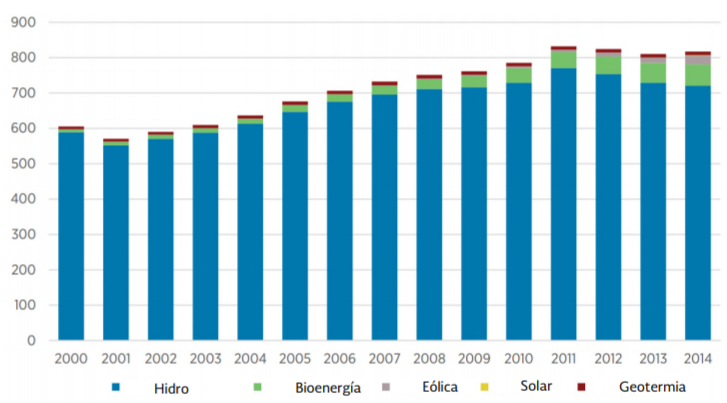
\includegraphics[width=10cm]{img/produccion.png}
	\caption{Evolución de la generación de electricidad en LatinoAmérica, 2000-2014. Fuente: Renewables in Latin American and the Caribbean, IRENA}
	\label{2000}
\end{figure}

\subsection{Las Energías Renovables en la Matriz Energética.}

La reducción en los costos, especialmente para la energía solar y eólica han permitido un considerable incremento en la participación de las energías renovables como fuentes de generación de energía limpia, aunado a esto, las políticas de apoyo para las energías renovables en México, derivadas de la Reforma Energética, han contribuido al fortalecimiento del mercado energético haciendo que las energías renovables sean altamente competitivas con los combustibles convencionales en el sector eléctrico.

\subsection{Potencial de Energías Renovables.}
El poder identificar zonas con alto potencial de energías renovables permite a los desarrolladores e interesados, invertir en proyectos que conlleven a la diversificación de la matriz energética.\\

De acuerdo al Inventario Nacional de Energías Renovables (INERE), el mayor potencial probado para generación de electricidad, es decir, aquel que cuenta con estudios técnicos y económicos que comprueban la factibilidad de su aprovechamiento, se encuentra en las energías eólica y solar.\\

El mayor potencial probable identificado, aquel que cuenta con estudios de campo que comprueban la presencia de los recursos, pero que no son suficientes para evaluar la factibilidad técnica y económica de explotación, corresponde a los recursos geotérmicos.\\

El mayor potencial posible se refiere al potencial teórico de los recursos pero que carece de los estudios necesarios para evaluar la factibilidad técnica y los posibles impactos económicos, ambientales y sociales. En este rubro el mayor potencial está en la energía solar seguida de la eólica.

\subsection{Avances en Energías Renovables}
Al cierre de 2015 la capacidad instalada de generación mediante energías renovables se incrementó 6.6\% respecto al periodo 2014, llegando a los 17,140.4 MW, lo cual representó el 25.2\% de la capacidad de generación total. La mayor parte de la capacidad en operación renovable continúa dominada por la generación hidroeléctrica, que en suma con la energía eólica representan el 80\% de la capacidad instalada en energías limpias. Entre 2005 y 2015, la energía eólica ha presentado la mayor expansión en capacidad instalada con el 104.7\% anual. Sin embargo, la energía hidráulica presenta la mayor concentración en la participación total de capacidad instalada con fuentes renovables, pero ha mantenido un ritmo de crecimiento de 1.7\% anual, como se muestra en la figura \ref{instalacion} a continuación.

\begin{figure}[!h]
	\centering
	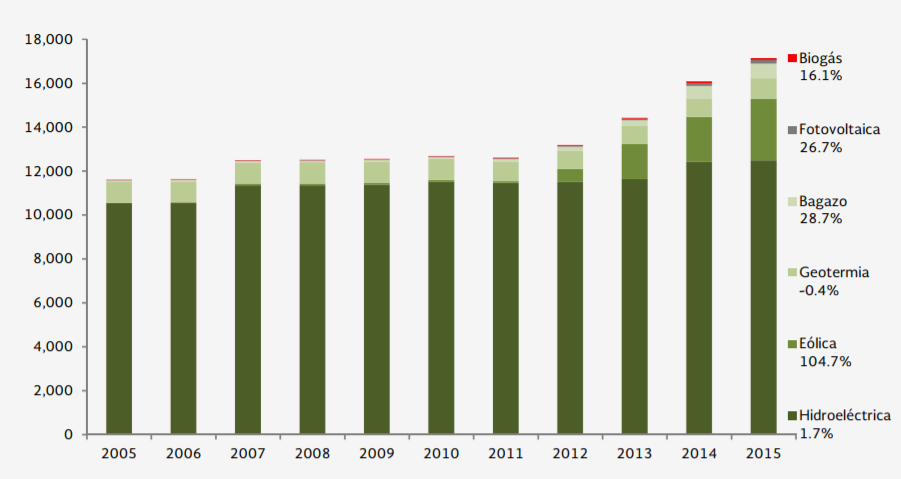
\includegraphics[width=10cm]{img/instalacion.png}
	\caption{Evlución de la capacidad instalada con enrgías renovables, 2005-2015.Fuente: SENER}
	\label{instalacion}
\end{figure}

\subsection{Generación Eléctrica con Energía Eólica.}
En los últimos cuatro años, la generación de energía eólica ha mostrado un crecimiento anual promedio equivalente a 2,330 GWh. Al cierre del 2015 la capacidad instalada alcanzó los 2,805.1 MW, lo que significó un incremento del 37.75\% respecto del 2014. En 2015, la generación eólica fue de 8,745.1 GWh, 36.08\% mayor a la generada en 2014. La generación de energía eléctrica a través de la energía eólica ha crecido significativamente desde 2005, de 5.0 GWh/año a 8,745.1 GWh, lo que representa un incremento de cerca del 174,802.0\%, clasificándose así en la segunda fuente de generación renovable (véase figura \ref{eolica}).

\begin{figure}[!h]
	\centering
	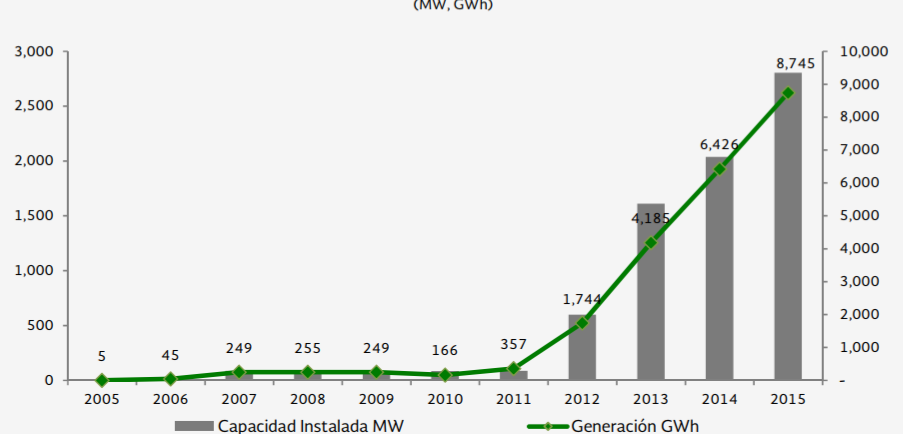
\includegraphics[width=10cm]{img/eolica.png}
	\caption{Capacidad instalada y generaciòn bruta de centrales eólica, 2005-2015. Fuente SENER}
	\label{eolica}
\end{figure}

\subsection{Generación Eléctrica con Energía Solar Fotovoltaica.}
Desde la publicación del Primer Contrato de Interconexión para Fuente de Energía Solar en Pequeña Escala, así como la entrada en operación de la primera central fotovoltaica de gran escala en 2011, la capacidad instalada y la generación de energía eléctrica a partir de energía solar se incrementó de 18.5 MW y 8.8 GWh en el año 2007 a 170.24 MW y 190.26 GWh en el año 2015. Este incremento se ha visto reforzado por el crecimiento importante de los Contratos de Interconexión Legados (Pequeña y Mediana Escala), los cuales desde 2010 han observado tasas de crecimiento importantes. (véase figura \ref{solar}).

\begin{figure}[!h]
	\centering
	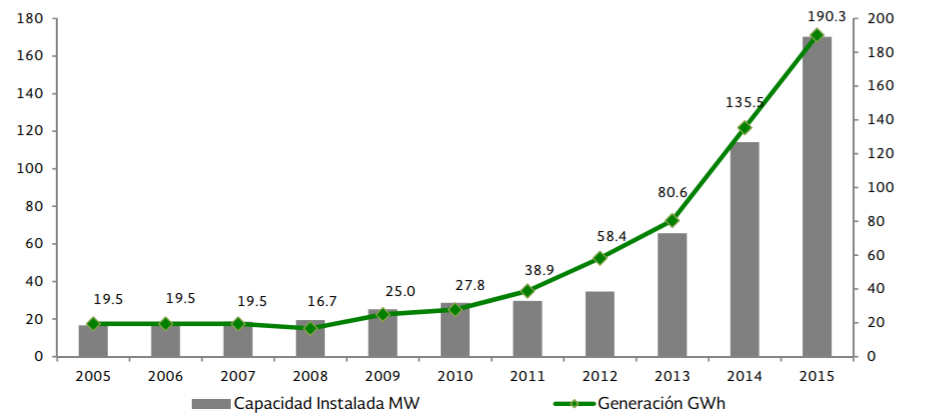
\includegraphics[width=10cm]{img/solar.png}
	\caption{Capacidades instaladas y generación bruta de centrales solares fotovoltaicas, 2005- 2015. Fuente: SENER}
	\label{solar}
\end{figure}

\section{Power TAC(Trading Agent Competition).}

Power TAC es una competencia de simulación de futuros mercados minoristas de energía eléctrica, en los que los competidores \textit{``broker''} o agentes minoristas (en la simulación son agentes inteligentes) que compran y venden energía tanto en los mercados mayoristas como minoristas. 
El mercado al por mayor es una abstracción de los típicos mercados diurnos en Norteamérica y Europa, y el mercado al por menor es un mercado de tarifas, en el que los clientes pueden elegir entre ofertas de contratos de tarifas ofrecidos por los agentes. Los clientes son modelos de usuarios domésticos, empresariales e institucionales de energía eléctrica, así como pequeños productores de energía que poseen paneles solares o turbinas eólicas.\\

Los brokers ofrecen servicios de energía a los clientes a través de contratos tarifarios, y luego deben servir a esos clientes negociando esa energía en el mercado al por mayor. En la competencia los brokers son desafiados a maximizar sus ganancias comprando y vendiendo energía en los mercados mayorista y minorista, sujetos a costos fijos y restricciones, el ganador de un juego o simulación individual es el broker con el saldo bancario más alto al final de la simulación \cite{WKetterJCollinsyMdWeerdtThe2017PowerTAC}.

La primera competencia de Power TAC se celebro en año 2012 como parte de la decimotercera competencia anual de agentes de comercio, durante la conferencia de AAMAS-12\footnote{The International Conference on Autonomous Agents and Multi-Agent Systems es la conferencia científica líder para la investigación en las áreas de inteligencia artificial, agentes autónomos y sistemas multiagentes.}. 
Los participantes diseñaron agentes  que actuaban como minoristas, obteniendo ganancias mediante la creación contratos y el comercio en el mercado al por mayor. 
El entorno  de simulación proporcionaba una gama de problemas para los agentes, incluyendo un mercado de energía al por mayor para el día a día, pronósticos de tiempo realistas que afectan la producción de energía eólica y solar, así como el consumo, una variedad de preferencias sobre términos de tarifas y un distribuidor de utilidades que cobra por el transporte de energía y por desequilibrios entre la oferta y la demanda.\\

Una segunda ronda de Power TAC 2012 se celebró del 24 al 27 de septiembre de 2012, y la tercera ronda se celebró del 30 de noviembre al 7 de diciembre. Posteriormente las competencias se fueron realizando cada año con diferentes participantes (véase la tabla \ref{tab:competition}).

\begin{table}[!h]
	\begin{center}
		\begin{tabular}{|p{1cm}|p{7cm}|p{4cm}|}\hline
			\textbf{Año} & \textbf{Participantes} & \textbf{Ranking} \\ \hline
			2013
			&
			\begin{tabular}{p{7cm}}
			Aston University\\
			University of Zagreb\\
			INAOE\\
			University of Freiburg\\
			Aristotle University of Thessalonik\\
			UT Austin\\
			CWI Amsterdam\\
		\end{tabular}
		&
		\begin{tabular}{p{4cm}}
			1 TacTex         \\
			2 cwiBroker      \\
			3 MLLBroker      \\
			4 CrocodileAgent \\
			5 AstonTAC       \\
			6 Mertacor       \\
			7 INAOEBroker02  \\
		\end{tabular}
		\\ \hline
																						
		2014
		&
		\begin{tabular}{p{7cm}}
			Universitaet Duisburg-Essen          \\
			University of Zagreb                 \\
			Westfaelische Hochschule             \\
			Aristotle University of Thessaloniki \\
			UT Austin                            \\
			INAOE                                \\
			CWI Amsterdam                        \\
		\end{tabular}
		&
		\begin{tabular}{p{4cm}}
			1 AgentUDE       \\
			2 cwiBroker      \\
			3 CrocodileAgent \\
			4 Maxon          \\
			5 Mertacor       \\
			6 coldbroker     \\
		\end{tabular}
		\\ \hline
																		
		2015
		&
		\begin{tabular}{p{7cm}}
			Universitaet Duisburg-Essen          \\
			INAOE                                \\
			The Chinese University of Hong Kong  \\
			University of Zagreb                 \\
			Westfaelische Hochschule             \\
			Aristotle University of Thessaloniki \\
			Nanyang Technological University     \\
			UTEP/NMSU                            \\
			Hebrew University of Jerusalem       \\
			UT Austin                            \\
			CWI Amsterdam                        \\
		\end{tabular}
		&
		\begin{tabular}{p{4cm}}
			1 Maxon15         \\
			2 TacTex          \\
			3 CUHKTac         \\
			4 AgentUDE        \\
			5 Sharpy          \\
			6 COLDPower       \\
			7 cwiBroker       \\
			8 Mertacor        \\
			9 NTUTacAgent     \\
			10 SPOT           \\
			11 CrocodileAgent \\
		\end{tabular}
		\\ \hline
																	
		2016
		&   
		\begin{tabular}{p{7cm}}
			The Chinese University of Hong Kong  \\  
			Universitaet Duisburg-Essen          \\
			INAOE                                \\
			University of Zagreb                 \\
			Aristotle University of Thessaloniki \\
			UTEP/NMSU                            \\
			Westfaelische Hochschule             \\
		\end{tabular}
		&
		\begin{tabular}{p{4cm}}
			1 maxon16        \\
			2 COLDPower      \\
			3 AgentUDE       \\
			4 SPOT           \\
			5 Mertacor       \\
			6 AgentCU        \\
			7 CrocodileAgent \\
		\end{tabular}
		\\ \hline
																								
		\end{tabular}			
	\end{center}
	\caption{Competencias realizadas por Power TAC 2013-2017.}
	\label{tab:competition}
\end{table}

El entorno de simulación de Power TAC modela un mercado  minorista y mayorista, una entidad de distribución y regularización y una población de clientes de producción y de consumo, situado en una ubicación real en la Tierra durante un periodo especifico con datos meteorológico reales. 
El mercado al por mayor es un mercado de llamadas relativamente simple, similar a muchos de los mercados ya existentes de energía eléctrica. 
Los modelos clientes incluyen hogares, vehículos electrónicos y entidades comerciales e industriales, además algunos de los clientes tienen capacidades de producción a partir de paneles solares y de turbinas eólicas. 
El distribuidor de utilidades modela un monopolio de regularización que posee  una red de distribución local y es responsable del mantenimiento de la infraestructura. 
El balance entre la oferta y la demandad en tiempo real es gestionado por un mecanismo basado en un mecanismo de incentivos económicos para alentar a los broker a mantener un equilibrio dentro de su portafolio de clientes de producción y de consumo. En la figura \ref{entorno} muestra los componentes principales que integra el entorno de simulación de PowerTAC.

\begin{figure}[!h]
	\centering
	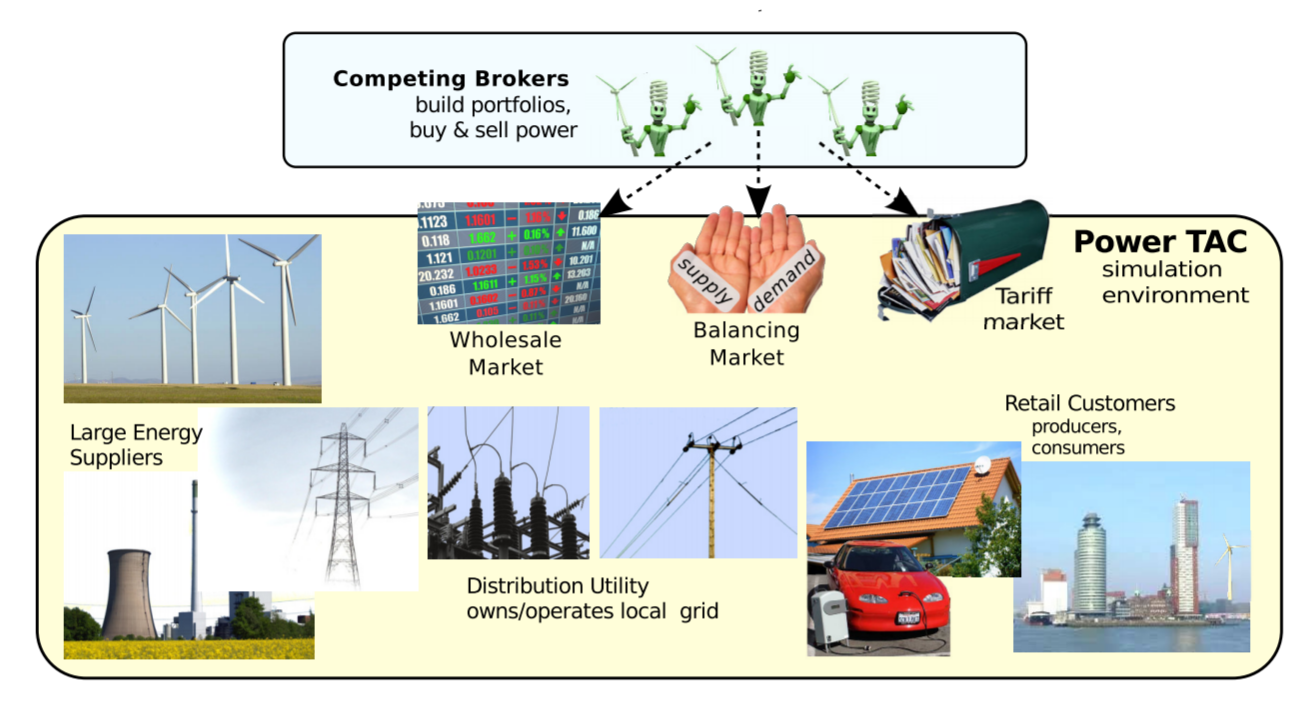
\includegraphics[width=10cm]{img/entorno.png}
	\caption{Elementos del entorno de simulación de Power TAC.}
	\label{entorno}
\end{figure}

A continuación se describen cada uno de los elementos:\\

\textbf{Customer Market.}\\

También conocido como el  Mercado de Tarifas, por este medio los agente adquiere energía eléctrica a través de los productores locales y posteriormente la vende a sus clientes de consumo. El agente adquiere clientes ofreciendo contratos o tarifas en el Mercado de Tarifas especificando el precio de la energía y otros términos, mientras que los clientes toman la decisión de aceptarlos o ignorarlos. 
Los paramentos que una tarifa permite especificar son los siguiente términos: periodo de pagos, tiempo de uso, bonos o pagos por suscripción, mínima duración de contrato, pagos de penalización de retiro antes de cumplir con la mínima duración, precio por consumo y producción, etc. Para más información  de la estructura de un tarifa véase la sección \ref{sec:tariff}.

\textbf{Wholesale Market.}\\

Mercado al por Mayor permite a los broker comprar y vender energía entre 1 y 24 horas en el futuro, por este razón también es conocido como Mercado del Día Siguiente. El broker y otros participantes proporcionan energía al por mayor a granel y liquidez al mercado, simulando la demanda de un mercado regional que es sustancialmente mayor que la demanda representada por el escenario de simulación de Power TAC.\\

\textbf{Distribution Utility.}\\

El Distribuidor de Utilidades (DU) modela el monopolio regulador y mantiene la infraestructura de distribución de energía. Dentro del contexto de Power TAC participa en los siguientes escenarios:

\begin{enumerate}
	\item Encargado de distribuir la energía de la red a los clientes, implicando pagos por el uso de la distribución de la energía hacia los clientes.
	\item Permite importar y exportar energía desde el Mercado al por Mayor.
	\item Actúa como broker de última instancia, ofreciendo sencillas tarifas clientes de consumo y de producción de energía.
	\item Participa en el proceso de balance de la red.
\end{enumerate}

\textbf{Balancing Market.}\\

El mercado de balance es el encargado de mantener el equilibrio entre la oferta y la demanda en la distribución en la red. 
El Mercado de Balance mantiene un sistema de incentivos para los broker por mantener el equilibrio entre la oferta y la demanda de su portafolio de clientes en cada intervalo de tiempo.\\

\textbf{Accounting.}\\

Para garantizar la coherencia y la imparcialidad, el simulador de Power TAC mantiene un registro de las cuentas de los agentes, las suscripciones de los clientes y las posiciones en el Mercado al por Mayor. Además mantiene un registro de las siguientes transacciones:

\begin{itemize}
	\item Suscripción y retiro de clientes por tarifa.
	\item Consumo y producción de energía por cliente.
	\item Pagos por publicación de tarifas.
	\item Pagos por distribución.
	\item Pagos del Mercado al por Mayor.
	\item Pagos del Mercado de Balance.    
\end{itemize}

Cada agente tiene una cuenta en efectivo en el banco central, e inicia el juego con un saldo de cero en la cuenta. Los créditos y débitos de las distintas transacciones se agregan a la cuenta durante cada timeslot.\\

\textbf{Weather reports.}\\

El pronóstico meteorológico y las condiciones meteorológicas actuales se envían a los brokers en cada intervalo de tiempo. Algunos modelos de clientes utilizarán esta información para influir en el consumo de energía y en la producción. Los informes meteorológicos y las predicciones se extraerán de los datos meteorológicos y de pronósticos del mundo real para hacerlo lo más realista posible. La ubicación específica y el intervalo de fechas para el conjunto de datos meteorológicos son información privilegiada, no revelada a los agentes, sin embargo se dan la latitud y época del año.\\

\textbf{Tiempo de simulación.}\\

El tiempo de simulación en Power TAC se divide en unidades de tiempo llamadas \textit{timeslot}, cada uno con una duración de una hora en tiempo de simulación y 5 segundos aproximadamente en tiempo real, es decir, que cada 5 segundos el servidor PowerTAC habra simulado una hora de eventos en un mercado energético.
Las rondas de simulación consisten en 60 días de simulación equivalente a 1440 timeslot o aproximadamente a 2 horas en tiempo real.\\

\section{Broker.}

El broker es el responsable de ser el intermediario entre las negociaciones en el Mercado de Tarifas, Mercado al por Mayor y el Mercado de Balance, con el objetivo de lograr ganancias a partir de la compra y venta de energía. Durante un times slot el agente puede realizar algunas de las actividades de la figura \ref{fig:activity}.

\begin{figure}[!h]
	\centering
	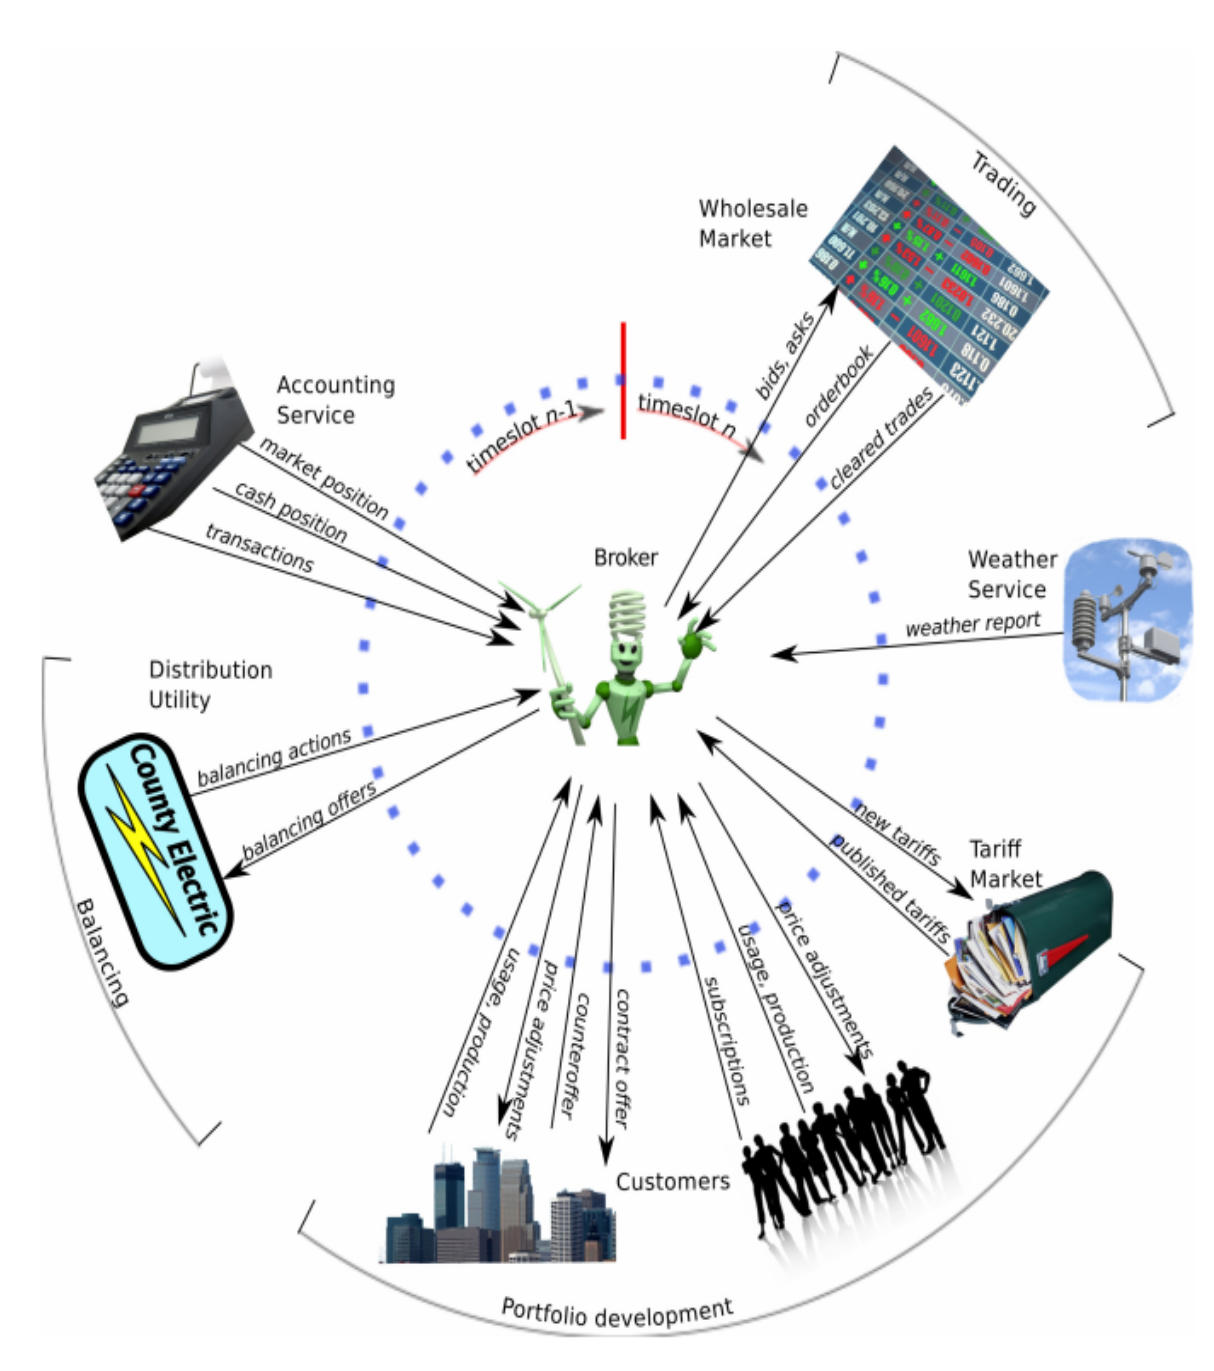
\includegraphics[width=8cm]{img/process.png}
	\caption{Actividades realizadas por el broker en un time slot.}
	\label{fig:activity}
\end{figure}

\begin{description}
	\item [Oferta de tarifas (Mercado de Tarifas):] crea y publica nuevas tarifas.
	\item [Modificación de tarifas (Mercado de Tarifas):]  cambia las condiciones de una tarifa reemplazandola por una nueva.
	\item [Ajuste de precios (Clientes):] ajustar los precios de las tarifas ya existentes.
	\item [Recortar la demanda (Clientes):] para los clientes que han suscrito a las tarifas que permiten capacidades controlables, los broker pueden ejercer restricciones para gestionar la demanda.
	\item [Publicar órdenes de balance (Mercado de Balance):] proporcionar al mercado de balance clientes con capacidades controlables para contribuir al desbalance de la red.
	\item [Enviar solicitudes y ofertas (Mercado al por Mayor):]  crear solicitudes y ofertas para vender y adquirir energía para los futuros timeslot.
\end{description}
\section{Customer.}

Power TAC ofrece modelos de clientes que interactúan con los broker mediante el Mercado de Tarifas. Cada uno de los clientes se caracteriza por un comjunto de información que incluye:

\begin{description}
	\item[Name:] un identificador único.
	\item[Population:] un entero representando el número de entidades indivisibles (casa, oficinas, vehículos eléctricos).
	\item[PowerType:] indica si el cliente es de producción o de consumo, además indica si  son controlables o de almacenamiento.
	\item[Controllable capacity:] son indicado por tres atributos: controlableKW  es el total de capacidad en kWh, up-regulation un rango máximo de descarga en kW y down-regulation un rango de máximo en kW de almacenamiento. Si estos tres números están en cero indica que este cliente no tiene capacidades controlables.
	\item[MultiContracting:] es la capacidad del cliente en particionar la población sobre múltiples tarifas.
	\item[CanNegotiate:] este campo indica que el cliente tiene la capacidad de negociar contratos individuales. Este campo por el momento no tiene utilidad para la competencia del 2017.
\end{description}

Cada uno de los clientes representa una población de clientes con características similares, los modelos de clientes realizan tres funciones básicas en el simulador:

\begin{itemize}
	\item Consumen y producen energía.
	\item Evalúan y se suscriben  a tarifas en el mercado de tarifas.
	\item Contribuyen a la demanda de la red, mediante la interrupción o  a la regularización (up-regulation o down-regulation).	
\end{itemize}

\subsection{Storage model.}
Representa un dispositivo de almacenamiento de energía con capacidad para controlar remotamente la carga y/o descarga. Este modelo permite representar el dispositivo de almacenamiento como las baterías, pero también permite representar otros dispositivos de almacenamiento por ejemplo dispositivos de almacenamiento térmico. Aunque la diferencia básica entre una batería y un dispositivo de almacenamiento térmico es que el dispositivo de almacenamiento térmico no puede descargarse para obtener energía eléctrica, pero su calor se utiliza para algún propósito (como calefacción, por ejemplo).

\subsection{Capacidades Controlables.}
Capacidades controlables o gestión de la demanda se puede presentar en dispositivos para clientes de producción y de consumo. 
Los clientes pueden proporcionar a los brokers diferentes formas de capacidades de gestión de la demanda que se pueden utilizar para controlar los costos o para equilibrar, según lo determinado por el PowerType. Estos difieren en la disponibilidad y la cantidad de energía disponible en un intervalo de tiempo. Algunos proporcionan regulación positiva (reducción de la demanda o aumento de la oferta), y algunos proporcionan regulación a la baja. Los dispositivos controlable en general son de dos tipos: 
\begin{enumerate}
	\item Dispositivos que permiten la interrupción del consumo o producción durante un rango asignado.
	\item Dispositivos con características de almacenamiento.
\end{enumerate}

Tres entidades interactúan con el fin de exponer, operar, evaluar y controlar las capacidades controlables: Los clientes, el Broker y el Distribuidor de Utilidades.\\

\textbf{Cliente.}\\

Algunos clientes ofrecen recursos que pueden ser controlables, y tienen preferencias sobre la conveniencia y precios de energía que afectarán su evaluaciones de las tarifas que proponen ejercer controles.\\

\textbf{Broker.}\\

Los broker pueden estar motivados a crear tarifas para clientes con capacidades controlables o de almacenamiento por las siguientes dos razones:

\begin{enumerate}
	\item Para reducir los costos en el Mercado al por Mayor. Un agente puede ejercer directamente controles para un intervalo de tiempo específico. Estos controles se denominan controles económicos.
	\item Para reducir los cargos por penalización durante el proceso de balance, el broker puede autorizar el DU a ejercer controles sólo en caso de hacerlo sería beneficioso para el broker. Tales controles se denominan controles de balance.
\end{enumerate}

\textbf{Distribuidor de Utilidades.}\\

El DU es el responsable de ejercer efectivamente los dispositivos con capacidades controlables, ya que controla la infraestructura física. Los controles de balance se ejercen después de la ejecución de los modelos de cliente, lo que significa que el DU debe comunicar un mensaje de control a los broker afectados, así como a los clientes. También debe emitir transacciones de tarifas adicionales para cada suscripción de la tarifa afectada.

\section{Tarifas.} \label{sec:tariff}
Las tarifas son la relación existente entre un broker y sus clientes, es decir es un contrato que especifica una serie de condiciones asociadas al precio, mínima duración de contrato, bonos y pagos por suscripción, etc. Los broker son los encargados de crear tarifas específicas a partir de un estructura definida  en la figura \ref{fig:tariff}. La estructura de una tarifa puede variar dependiendo al PowerType que esté sujeta a ella.

\begin{figure}[!h]
	\centering
	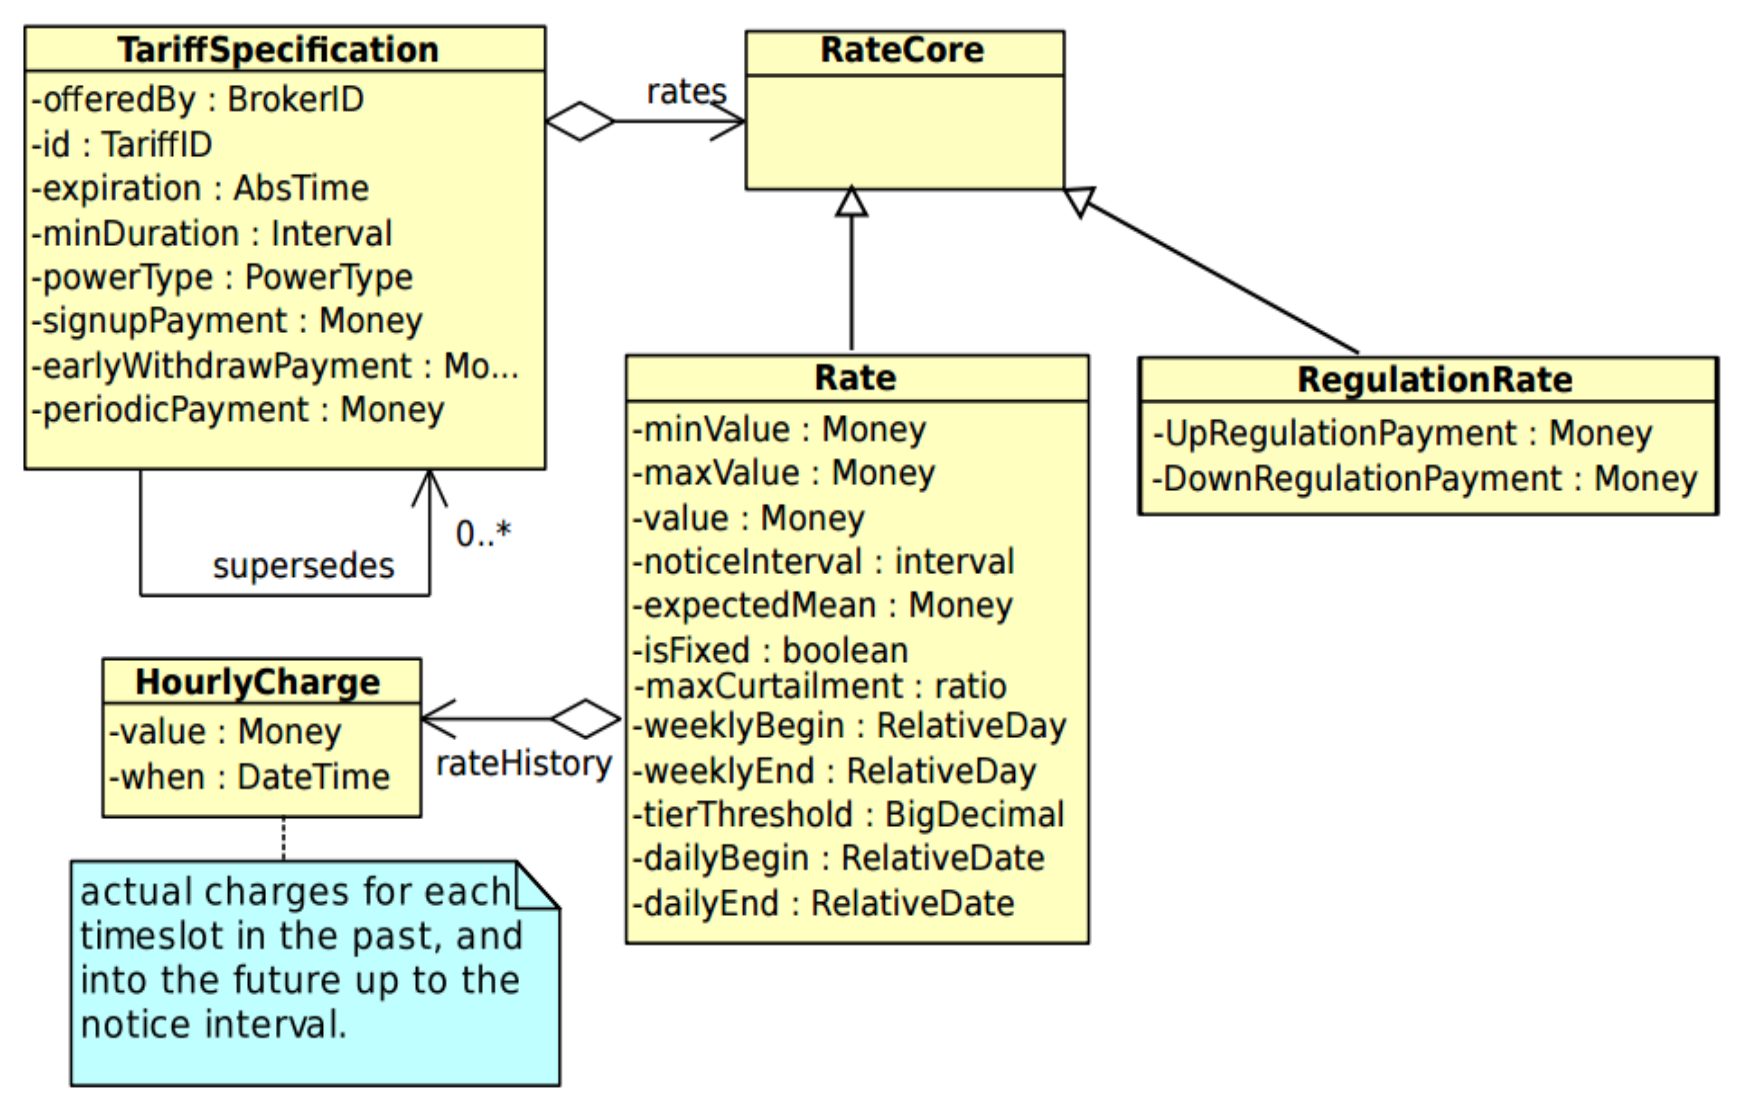
\includegraphics[width=13cm]{img/tariffstructe.png}
	\caption{Clases asociadas a la estructura de una tarifa.}
	\label{fig:tariff}
\end{figure}

Muchos de los elementos de una tarifa son representados por la estructura TariffSpecification donde podemos indicar las condiciones del pago y el PowerType, pero el precio de la energía es definido mediante la estructura Rate. La cantidad de dinero y de energía especificado en TariffSpecification es visto desde el punto de vista de un cliente, es decir  un valor es negativo representa una pago del cliente al broker, mientras un valor positivo representa un pago desde el broker al cliente. Similarmente una cantidad de energía representado en kWh con un valor positivo representa energía entregada al cliente y un valor negativo es la energía entregada al broker.\\

Cuando el broker publica una tarifa esta debe de pasar por una serie de estados, en la figura \ref{state} se muestran los estados de una tarifa. El broker envía una tarifa al mercado de tarifas y esta entra en estado de “pending”. Las nuevas tarifas son publicadas periódicamente a los clientes y a los broker, entrando al estado “Offered”, los clientes se suscriben y la tarifa entra en un estado “active”. Inmediatamente el broker es notificado de varios eventos entre ellos, suscripción de clientes, cancelación de contrato, entre otras acciones. Las tarifas pueden tener una fecha de vencimiento y no se permiten nuevas suscripciones en este caso entra en un estado de “expired” hasta que esta es revocada o modificado por un broker.

\begin{figure}[h!]
	\centering
	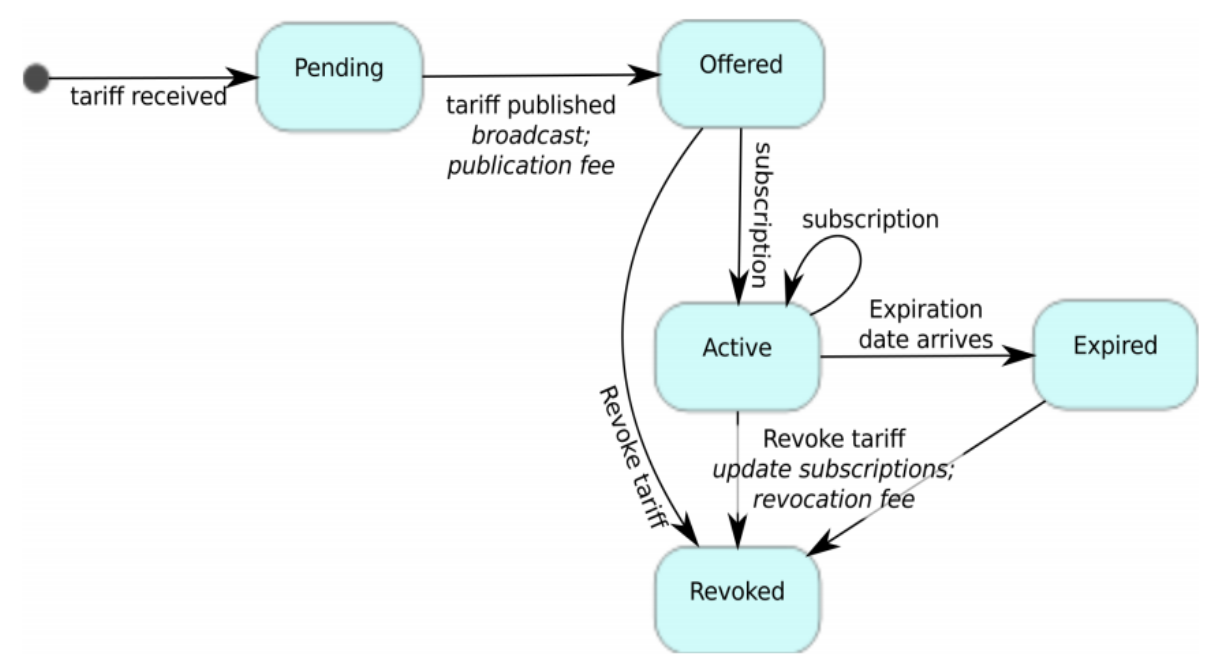
\includegraphics[width=10cm]{img/state.png}
	\caption{Estados de un tarifa.}
	\label{state}
\end{figure}

\subsection{Tarifas para clientes con capacidades controlables.}

Los clientes con capacidades controlables pueden elegir tarifas especificas diseñadas para proporcionar control en los dispositivos o pueden optar por tarifas más generales que no proporcionen un control sobre ellos. 
La cuestión es como el cliente obtiene beneficios por permitir un control externo. 
Con los dispositivos de consumo controlable estándar los clientes obtienen un descuento en la tasa de consumo a cambio de permitir la reducción del consumo. 
Pero este esquema no parece adecuado para clientes con dispositivos de almacenamiento, una solución es pagar o cobrar al clientes por las acciones de carga y descarga de sus dispositivos. 
En la construcción de una tarifa para clientes con capacidades controlables se puede incluir términos de interrupción y de regularización a partir de una estructura externa a TariffSpecification, empleando la estructura Rate y RegulationRates definimos los términos antes mencionados. 
Los clientes interrumpibles permiten que una porción de consumo o producción del cliente se reduzca durante una porción del intervalo de tiempo para reducir los costos generales de energía y para reducir costos del desbalance. 
La estructura de RegulationRates permite incluir un valor para especificar un tasa de interrupción durante un timeslot, agregando un valor distinto de cero en la propiedad de maxCurtaiment dentro de la estructura del Rate. 
Para los cliente con capacidades de almacenamiento, dentro de la estructura RegulationRates se puede incluir términos para los pagos por el uso del dispositivo durante un desbalance negativo (up-regulation) o un desbalance positivo (down-regulation).

\section{Información disponible para los brokers.}

El servidor de Power TAC durante un juego proporciona información del entorno de simulación a los broker, esta información es enviada a partir de mensaje  asíncronos y puede ser pública o privada.\\

Al inicio de la simulación el broker recibe la siguiente información:
\begin{description}
	\item [Game parameters: ]Parámetros usados para la configuración o instancia de un juego específico.    
	\item [Broker Identities: ]\textit{Username} de los broker participantes en el juego.
	\item [Customer Records: ]Nombres y características de los modelos de clientes ejecutados durante la simulación.
	\item [Default tariff: ]Al iniciar el juego, el mercado de tarifas solo oferta tarifas publicadas por el default broker.
	\item [Bootstrap Customer Data: ]Consumo y producción de cada uno de los clientes durante un periodo de 14 días antes de iniciar la simulación.
	\item [Bootstrap Market Data: ]Precios y cantidades de energía comprada por el Default Broker en el Mercado al por Mayor durante los 14 días anteriores al inicio de la simulación.
	\item [Bootstrap Weather data: ]Reportes del clima durante los 14 días antes del inicio de la simulación.
	\item [Weather report, Weather forecast: ]Predicciones del clima en las siguientes 24 horas.  
\end{description}
La siguiente información se envía a los brokers una vez cada 6 horas de simulación, cuando se publican las tarifas:
\begin{description}
	\item [Tariff updates: ]Las siguiente acciones, creación de nuevas tarifas, revocación de tarifas y sustitución de tarifas, se les notificará a cada uno de los brokers.
	\item [Tariff transactions:] Cuando se publica una tarifa de un broker, se  cobra un bono por publicación, cuando los clientes  cambian la suscripción, los broker reciben transacciones que describen los cambios junto con una bonificación o una cantidad de penalizaciones de salida anticipada. Esta información es privada y solo para el propietario de la tarifa.
\end{description}
La siguiente información es pública y se envía a cada uno de los broker en cada time slot.
\begin{description}
	\item [Wholesale market clearing data: ]Los precios de compensación del mercado y las cantidades totales negociadas para cada una de las 24 oportunidades de negociación en el Mercado al por Mayor. Estos mensajes pueden omitirse si no se hicieron operaciones en un intervalo de tiempo dado.
	\item [Wholesale market orderbooks: ]Contiene precios y cantidades de todas las ofertas y solicitudes no satisfechas.
	\item [Total aggregate energy consumption: ]Producción y consumo total de energía para el intervalo de tiempo actual.
	\item [Wheather report and weather forecast:] Condiciones meteorológicas para el intervalo de tiempo actual y pronóstico para las próximas 24 horas.
\end{description}
Cada vez que se ejecuta la evaluación de demanda máxima una vez por semana, cada broker recibirá un conjunto de mensajes de Capacity transactions, una para cada pico de demanda evaluado. Estas transacciones especifican el umbral de demanda, la contribución del broker al pico de energía y la cuota asociada. La siguiente información es privada y enviado individualmente a cada broker en cada time slot.
\begin{description}
	\item [Tariff transactions:] Lecturas de créditos y débitos asociados a los clientes.
	\item [Balancing and distribution transactions:] Cargos por el DU para cada broker individual para compensar el Mercado de Balance y la distribución de energía.
	\item [Portafolio supply and demand:] Transacciones de producción y consumo de los clientes actuales del broker.
	\item [Wholesale market transations:] Ofertas y peticiones presentadas por el broker.
	\item [Market Positions:] Los compromisos netos actualizados de importación / exportación del Broker, para cada una de las 24 oportunidades de negocio en el Mercado al por Mayor.
	\item [Cash Position: ]Actualización de la cuenta bancaria del Broker después de que todas las transacciones contables vigentes se han aplicado.
\end{description}

\section{Wholesale Market.}

En el mercado al por mayor los brokers interactúan entre si directamente así como con grandes compañías productoras y otros participantes del mercado al por mayor vendiendo y comprando grandes cantidades de energía, la cual usan para venderla en el mercado al por menor (mercado de tarifas). 

En el mercado al por mayor los agentes pueden negociar energía través de órdenes de compra o venta para una hora determinada (hora objetivo) en cualquiera de las 24 horas anteriores. Estas órdenes pueden o no ser ejecutadas, en dependencia del precio de cruce del mercado, el cual es calculado a partir de los precios de compra y ventas de todas las órdenes recibidas por el mercado \cite{WKetterJCollinsyMdWeerdtThe2016PowerTAC}.

En este mercado la energía es más cara que en el mercado de tarifas ya que tiene una mayor estabilidad, por lo que se debe de evitar lo más posible. Los clientes son modelos de usuarios empresariales e institucionales de energía eléctrica, así como grandes productores de energía.

\section{Balance Market.}

El Mercado de Balance debe satisfacer tres objetivos:
\begin{enumerate}
	\item El consumo total de energía neta debe sumar a cero una vez que el mercado se ha liquidado.     
	\item Cada broker que tiene un balance positivo debe tener clientes de producción controlables cuya producción poder reducir o clientes de consumo controlables (como baterías) cuyo consumo poder aumentar para poder disminuir el balance positivo, o debe pagar por su exceso de energía por una tasa determinada por el proceso de balance del mercado.
	\item Cada broker que tiene un balance negativo debe tener clientes de consumo controlables cuyo consumo poder disminuir, o clientes de producción cuya producción poder aumentar (las baterías y los autos eléctricos también pueden regresar energía a la red) o debe pagar por la energía adicional necesaria.
\end{enumerate}

\section{Distribuidor de Utilidades.}
El DU opera la red de distribución que conecta la red de transmisión al por mayor de los agentes y clientes. También actúa como el “agente por defecto", ofreciendo tarifas básicas y poco atractivas para todos los tipos de clientes. 
Los  costos del DU deben ser cubiertos por los honorarios pagados por los agentes a través de las comisiones de distribución y de regularización. 
Con capacidad controlable, los broker pueden presentar órdenes de balance que le permiten al DU ejercer control de capacidad para lograr el equilibrio. 
Los brokers deben presentar sus órdenes de balance antes de que se ejecuten los modelos de cliente y el DU ejecuta su proceso de balance después de que se conozca el consumo del cliente para el intervalo de tiempo actual. 
El DU puede determinar las cantidades reales disponibles para cada orden de balance.
\\
\section{Regresión}
En estadística, el análisis de la regresión es un proceso estadístico para estimar las relaciones entre variables. Incluye muchas técnicas para el modelado y análisis de diversas variables, cuando la atención se centra en la relación entre una variable
dependiente y una o más variables independientes (o productoras, o regresoras).
Más específicamente, el análisis de regresión ayuda a entender cómo el valor de la variable dependiente varía al cambiar el valor de una de las variables independientes, manteniendo el valor de las otras variables independientes fijas \cite{BoundlessRegressionAnalysis}.

El análisis de regresión es ampliamente usado para predicción, donde tiene una superposición con el área de machine learning. 
El análisis de regresión también es usado para entender cuáles de las variables independientes está relacionada a la variable dependiente, y explora las formas de estas relaciones. 
En algunas circunstancias, el análisis de regresión puede ser usado para inferir relaciones causales entre las variables dependiente e independiente \cite{BoundlessRegressionAnalysis}, sin embargo, esto puede llevar a falacias de relación, por ejemplo ``\textit{Cum hoc ergo propter hoc}'' (en latín, ``con esto, por tanto a causa de esto'', o también conocida como ``correlación no implica causalidad'') \cite{JSArmstrongIllusions}.

\subsection{Regresión lineal}

La regresión lineal es el tipo más básico de regresión y es comúnmente usado en el análisis predictivo.
Es un enfoque para modelar la relación entre una variable dependiente escalar, y una o más variables independientes (también llamadas predictoras) denotadas por $X$. 
En el caso de que el modelo de regresión solo tenga una variable independiente es llamado \textit{regresión lineal simple}, para más de una variable predictora, el proceso es llamado regresión lineal múltiple \cite{DAFreedmanStatisticalModels}, este término es distinto de regresión lineal multivariable donde múltiples variables dependientes correlacionadas son predichas, en lugar de una sola variable escalar \cite{ACRencherWFChristensenMethods}.

Más formalmente, dado un conjunto de datos $\{y_i,x_{i1},...,x_{ip}\}_{i=1}^n$ de $n$ unidades estadísticas, un modelo de regresión lineal asume que la relación entre la variable dependiente $y_i$ y el p-vector de variables $x_i$ es lineal. Esta relación es modelada
con un término de perturbación o variable de error $\varepsilon_i$, una variable aleatoria no observada que agrega ruido a la relación lineal entre la variable dependiente y las variables regresoras, la figura \ref{ec:regresionLineal} contiene la ecuación que representa el modelo de regresión lineal.

\begin{figure}
\[ y_i= \beta_0 + \beta_1x_{i1} +...+ \beta_px_{ip} + \varepsilon_i \]
\caption{Ecuación de un modelo lineal}
\label{ec:regresionLineal}
\end{figure}

\begin{enumerate}
	\item $y_i$ es llamada la variable dependiente, variable criterio, variable de respuesta o variable medida. La decisión de cual variable del conjunto de datos es modelada como la variable dependiente puede basarse en una suposición de que el valor de una variable es causado o directamente influenciado por las otras variables.
	
	\item $x_{i1} + x_{i2}+...+x_{ip}$ son llamados variables independientes, regresoras, productoras o predictoras.
	\begin{enumerate}
		\item Usualmente una constante es incluida como una de las variables regresoras, por ejemplo, podemos decir que $x_{i1} = 1$ para  $i =1...n$.
		\item A veces uno de los regresores pueden ser funciones no lineales de otro regresor, como en la regresión polinomial (método el cual se usó para implementar regresión polinomial) y regresión segmentada, el modelo permanece lineal, siempre y cuando sea lineal en el vector de parámetros $\beta_p$.
	\end{enumerate}
	\item $\beta_p$ es un vector de parámetros, cuyos elementos, los coeficientes de regresión, son los valores buscados por la regresión.
	\item $\varepsilon_i$ es llamado el término de error o ruido. Esta variable representa todos los otros factores que influencian la variable dependiente, además de los regresores $x_{ip}$.
\end{enumerate}
\subsection{Regresión polinomial}

En estadística, la regresión polinomial es una forma de regresión lineal en la cual la relación entre la o las variables independientes esta modelada por un polinomio de las variables independientes de grado n.

En general podemos modelar el valor de la variable dependiente y como un polinomio de grado $n$ de las variables independientes, la ecuación de la figura \ref{ec:regresionPolinomial} es un ejemplo de un modelo con una sola variable independiente $x$:
 
\begin{figure}
\[ y_i=b_0 + b_1x + b_2x^{2}+...+b_nx^{n} \]
\caption{Ecuación de un modelo polinomial}
\label{ec:regresionPolinomial}
\end{figure}

La regresión polinomial encaja en los modelos no lineales ya que la relación entre las variables independientes y la dependiente es no lineal, al tratarse de un polinomio el que la describe.

Aunque la regresión polinomial se considera un modelo de datos no lineal, como un problema de estimación estadística es lineal, en el sentido de que los parámetros buscados por la función de regresión ($\beta_n$) son una combinación lineal de los términos del polinomio que representa el modelo. Por esta razón es considerado un caso especial de regresión lineal múltiple.

Para resolver un modelo de regresión polinomial, por ejemplo de una variable como en la ecuación de la figura \ref{ec:regresionPolinomial}, hay que expandir el modelo agregando variables independientes que son cada uno de los términos de grado $i$, para $i=1,2... n$, donde n es el grado del polinomio.
Las variables predictoras resultantes de la expansión polinomial del modelo base, son conocidas como características de interacción \cite{YWChangCJHsiehKWChangTrainingAndTesting}.

\subsection{Series de tiempo}
Una serie de tiempo es una secuencia de datos, que representan observaciones o mediciones de algún fenómeno, indexados por tiempo, más comúnmente, una secuencia de observaciones tomadas en puntos sucesivos en el tiempo igualmente espaciados. Por lo tanto es una secuencia de datos de tiempo discretos. 
Ejemplos de una serie de tiempo son la altura de las mareas cada hora, la tasa mensual de desempleo de los últimos 5 años, el valor de cierre diario de cierta empresa.

Las series de tiempo son muy frecuentemente ilustradas con gráficas de líneas. 
Son usadas en la estadística, procesado de señales, reconocimiento de patrones, matemática financiera, pronóstico climático, y en general en cualquier dominio de ciencia aplicada e ingeniería, que involucren mediciones temporales.

El análisis de series de tiempo comprende métodos para analizar datos de series de tiempo con el objetivo de extraer valores estadísticos útiles y otras características de los datos. 
El pronóstico de series de tiempo es, el uso de un modelo para predecir futuros valores basados en datos previamente observados. 
Mientras que el análisis de regresión es a menudo empleado de manera tal que pruebe teorías de que los valores actuales de una o más series de tiempo independientes afectan el valor actual de otra serie de tiempo, este tipo de análisis de series de tiempo no se llama
``análisis de serie de tiempo'', el cual se enfoca en comparar valores de una sola serie de tiempo o en múltiples series de tiempo dependientes en diferentes momentos del tiempo \cite{MImdadullahTimeSeriesAnalysis}.

Típicamente los autores reconocen 4 componentes básicos en una serie de tiempo, los cuales en conjunto (unidos de manera aditiva o multiplicativa) contribuyen a los cambios observados en un período de tiempo y dan a la serie su aspecto errático.
Los cuatro componentes básicos son: Tendencia secular, variación estacional, variación cíclica y variación irregular.

\section{Clasificación}

Una gran cantidad de enfoques se han tomado en esta tarea, tres ramas históricas principales de investigación se pueden identificar: estadística, \textit{machine learning} o aprendizaje automático y redes neuronales. 
En el aprendizaje automático y estadística, la clasificación es el problema de identificar a que conjunto de categorías pertenece una nueva observación, con base en un conjunto de datos de entrenamiento (training set) que contiene observaciones  (o instancias) cuyas pertenencias a las diferentes categorías es conocida.

Estas tres ramas han involucrado ampliamente diferentes grupos profesionales y académicos, y enfatizado diferentes problemas.
Sin embargo todos los grupos han tenido algunos objetivos en común, todos han intentado desarrollar procedimientos que puedan:

\begin{enumerate}
	\item Igualar o superar un comportamiento humano de toma de decisiones, pero con la ventaja de consistencia y a medida variable, explicidad.
	\item Manejar una gran variedad de problemas y, con suficientes datos, ser extremadamente general.
	\item Ser usado en entornos prácticos con éxito comprobado.
\end{enumerate}

\subsection{Enfoque estadístico}
El acercamiento estadístico a la clasificación es generalmente caracterizado por modelo probabilístico explícito subyacente, el cual provee una probabilidad de que una observación se encuentre en cada clase en lugar de una simple clasificación. Además es normalmente asumido que las técnicas serán usadas por estadísticos, y por lo tanto, algo de intervención humana es asumida con respecto a la selección y transformación de variables, y la estructuración general del problema.

\subsection{Aprendizaje automático}
El aprendizaje automático o machine learning generalmente se considera que abarca procedimientos automáticos de computación basados en operaciones lógicas o binarias, que aprenden una tarea a partir de una serie de ejemplos.
La atención se ha concentrado en enfoques de árboles de decisión, en la cual la clasificación resulta de una secuencia de pasos lógicos, estos son capaces de representar los problemas más complejos dados suficientes datos.
Otras técnicas como los algoritmos genéticos y procedimientos lógicos inductivos (ILP) están actualmente en desarrollo activo y en principio nos permitirían tratar con tipos de datos más generales, incluyendo casos donde el número y tipo de atributos puede variar, y donde capas adicionales de aprendizaje son superpuestas, con jerarquía estructural de atributos y clases y demás. 

El aprendizaje automático apunta a generar expresiones de clasificación lo suficientemente simples para ser entendidas fácilmente por un humano, estas deben imitar el razonamiento humano lo suficiente para proveer de pistas sobre el proceso de decisión. 
Como el enfoque estadístico, el conocimiento previo puede ser explotado en el desarrollo, pero en la operación se asume que se realiza sin intervención humana.

\subsection{Redes neuronales}
Una amplia clase de técnicas pueden caer dentro de este título, pero generalmente, las redes neuronales consisten en capas de nodos interconectados, cada nodo produce una función no lineal de su entrada. La entrada de un nodo puede venir de otros nodos o directamente de los datos de entrada. También, algunos nodos son identificados como la salida de la red. La red completa por lo tanto representa un muy complejo conjunto de interdependencias las cuales pueden incorporar cualquier grado de no-linealidad, permitiendo moldear funciones muy generales. 

El enfoque de redes neuronales combina la complejidad de algunas de las técnicas estadísticas con el objetivo del aprendizaje automático de imitar la inteligencia humana, sin embargo esto es hecho a un nivel más ``inconsciente'' y por lo tanto no hay una manera de hacer los conceptos aprendidos transparentes para el usuario \cite{Michie94machinelearning}.

\subsection{Árboles de decisión}
Un árbol de decisión es un modelo predictivo que puede ser usado para representar un modelos de clasificación y regresión. 
Los árboles de decisión se usan para clasificar objetos o instancias (como una persona asegurada) en un conjunto de clases predefinidas (tales como riesgoso/no riesgoso) basado en los valores de sus atributos (tales como edad, genero, etc.), midiendo el error de predicción en términos del numero de instancias erróneamente clasificadas \cite{RokachLiorMaimonDataMiningDecisionTrees}.
Los árboles de regresión son para variables dependientes que toman valores continuos o valores ordenados discretos, y sus errores de predicción típicamente se miden por el cuadrado de la diferencia entre el valor observado y el valor predicho. \cite{LohWei-YinClassificationAndRegressionTrees}


Es uno de los enfoques de modelado predictivo utilizados en estadísticas, minería de datos y aprendizaje automático. 
Los modelos de árbol, donde la variable de destino puede tomar un conjunto finito de valores se denominan árboles de clasificación. 
En estas estructuras de árbol, las hojas representan etiquetas de clase y las ramas representan las conjunciones de características que conducen a esas etiquetas de clase. 
Los árboles de decisión, donde la variable de destino puede tomar valores continuos (por lo general números reales) se llaman árboles de regresión. El aprendizaje basado en árboles de decisión es una de las técnicas más eficaces para la clasificación supervisada.

Un árbol puede ser ``aprendido'' mediante el fraccionamiento del conjunto inicial en subconjuntos basados en una prueba de valor de atributo. 
Este proceso se repite en cada subconjunto derivado de una manera recursiva llamada particionamiento recursivo. 
La recursividad termina cuando el subconjunto en un nodo tiene todo el mismo valor de la variable objetivo, o cuando la partición ya no agrega valor a las predicciones. 
Este proceso de inducción top-down de los árboles de decisión \cite{InductionofDecisionTrees1986}
es un ejemplo de un algoritmo voraz, y es, con mucho, la estrategia más común para aprender árboles de decisión a partir de datos.

\subsection{Método bagging}
La agregación bootstrap o bagging es un meta algoritmo para generar múltiples versiones de un predictor y con estos conseguir un predictor agregado. La agregación hace un promedio de todas las versiones cuando predice una salida numérica (comúnmente regresión) y hace una votación por mayoría cuando predice clases (clasificación).
Las multiples versiones se forman haciendo réplicas bootstrap de el conjunto de datos de entrenamiento y usando estas como nuevos conjuntos de entrenamiento.
Una réplica bootstrap de un conjunto de entrenamiento $D$ de tamaño $n$ se trata de un muestreo uniforme y con reemplazo de $D$, obteniendo un subconjunto $D'$ de tamaño $n'$. En el caso de muestreo con reemplazo algunas observaciones deben repetirse en $D'$. Si $n'=n$ entonces para un $n$ grande el conjunto $D'$ se espera que tenga $(1-1/e) \approx 63.2\%$ de ejemplos únicos de $D$ siendo el resto duplicados \cite{EstimatingtheSizeandConfidenceofaStatisticalAudit}.

Pruebas en conjuntos de datos reales y simulados usando árboles de regresión y clasificación y selección de subconjuntos en regresión lineal muestran que el metodo bagging puede dar ganancias substanciales en exactitud.
El elemento importante es la inestabilidad del método de predicción, si perturbar el dataset de entrenamiento puede causar cambios significativos en el predictor construido, entonces el metodo bagging puede mejorar la exactitud. Por otra parte, esto puede degradar levemente el rendimiento de métodos estables tales como K-nearest neighbors.
\cite{BreimanLMachineLearning1996}.

\subsection{Redes bayesianas}
Una red bayesiana es un modelo probabilístico representado en un grafo acíclico dirigido. Representa un conjunto de variables aleatorias y sus dependencias condicionales. Dado este modelo, se puede hacer inferencia bayesiana; es decir, estimar la probabilidad posterior de las variables no conocidas, en base a las variables conocidas \cite{LESucarChapter1RedesBayesianas}. 

Los nodos representan variables aleatorias en el sentido de Bayes. Cada nodo tiene asociado una función de probabilidad que toma como entrada un conjunto particular de valores de las variables padres del nodo y devuelve la probabilidad de la variable representada por el nodo. Las aristas representan dependencias condicionales.

Si por padres son m variables booleanas entonces la función de probabilidad puede ser representada por una tabla de $2^m$ entradas, una entrada para cada una de las $2^m$ posibles combinaciones de los padres siendo verdadero o falso.

En la \ref{fig:redBayesianaEjemplo} podemos ver un ejemplo de red bayesiana simple, el cual modela la probabilidad de tres eventos, las probabilidades de que llueva, que un rociador este activado, y que la hierba de un campo este húmeda. Hay dos eventos los cuales pueden causar que la hierba esté húmeda: que el rociador esté activado o que esté lloviendo, esta relación se representa mediante las aristas.

\begin{figure}[h!]
	\centering
	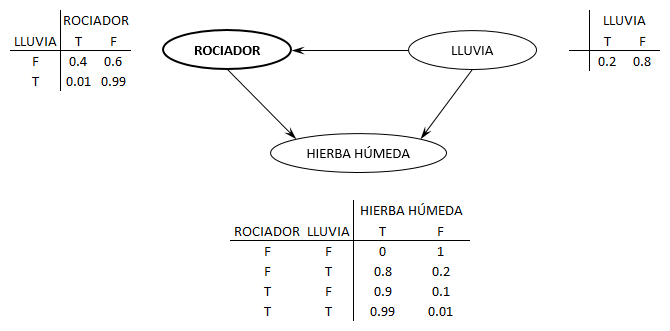
\includegraphics[width=8.75cm]{img/redBayesianaEjemplo.png}
	\caption{Ejemplo de red bayesiana simple.}
	\label{fig:redBayesianaEjemplo}
\end{figure}